\documentclass[a4paper,landscape,8pt]{extarticle}

\usepackage[a4paper,margin=0.7cm]{geometry}

\usepackage{fancyhdr}
\pagestyle{fancy}
\fancyfoot[R]{\vspace{-35pt}\Huge\thepage}

\usepackage{multicol}
\setlength\columnsep{20pt}
\setlength{\columnseprule}{0.1pt} 

\setlength\parindent{0pt}

\usepackage[ngerman]{babel} % Silbentrennung
\usepackage[utf8]{inputenc} % Umlaute
\usepackage{microtype}

\usepackage{hyperref}

\usepackage{float}
\usepackage{graphicx}

\usepackage{comment}

\usepackage{amsmath}
\usepackage{amssymb}

\usepackage{cancel}

\usepackage{color}
\usepackage[table]{xcolor}

\usepackage{color}

\usepackage{booktabs}

\newenvironment{rcases}
  {\left.\begin{aligned}}
  {\end{aligned}\right\rbrace}
  
\usepackage{enumitem}
\setlist{noitemsep,topsep=3pt,parsep=3pt,partopsep=3pt,leftmargin=18pt}
\renewcommand\labelitemi{{\boldmath$\cdot$}}
\newcommand{\listarrow}{
\smash{\scalebox{1.5}[1.75]{\rotatebox[origin=c]{180}{$\Lsh$}}}
}

\usepackage{xifthen}
\newcommand{\emptyarg}[1][]{\ifthenelse{\isempty{#1}}{}{\ (#1)}}

% % % % %
% Structural
% % % % %

\newcommand{\Def}[1][]{\colorbox{defcolor}{\color{titlecolor}{\textbf{Def.\emptyarg[#1]}}}\kern+0.3ex}

\newcommand{\Satz}[1][]{\colorbox{thmcolor}{\color{titlecolor}{\textbf{Thm.\emptyarg[#1]}}}\kern+0.3ex}

\newcommand{\Lemma}[1][]{\colorbox{thmcolor}{\color{titlecolor}{\textbf{Lem.\emptyarg[#1]}}}\kern+0.3ex}

\newcommand{\Korollar}[1][]{\colorbox{thmcolor}{\color{titlecolor}{\textbf{Kor.\emptyarg[#1]}}}\kern+0.3ex}

\newcommand{\Trick}[1][]{\colorbox{trkcolor}{\color{titlecolor}{\textbf{Trick:\emptyarg[#1]}}}\kern+0.3ex}

\newcommand{\Vorgehen}[1][]{\colorbox{trkcolor}{\color{titlecolor}{\textbf{Vorgehen:\emptyarg[#1]}}}\kern+0.3ex}

\newcommand{\Bsp}[1][]{\colorbox{bspcolor}{\color{titlecolor}{\textbf{Bsp.\emptyarg[#1]}}}\kern+0.3ex}

% % % % %
% In Text
% % % % %

\newcommand{\Bem}{\textbf{Bem: }}
\newcommand{\Beweis}{\textbf{Beweis: }}
\newcommand{\Achtung}{\textbf{Achtung: }}
\newcommand{\Wichtig}{\textbf{Wichtig: }}

% % % % %
% Colors
% % % % %

\definecolor{defcolor}{rgb}{0.75, 1, 0.75}
\definecolor{thmcolor}{rgb}{1, 0.75, 0.75}
%\definecolor{trkcolor}{rgb}{1, 0.7, 0}
\definecolor{trkcolor}{rgb}{0.7, 0.95, 1}
\definecolor{bspcolor}{rgb}{1, 0.95, 0.43}
\definecolor{titlecolor}{rgb}{0,0,0}

% % % % %
% Math
% % % % %

\DeclareMathOperator{\arcsinh}{arcsinh}
\DeclareMathOperator{\arccosh}{arccosh}
\DeclareMathOperator{\arctanh}{arctanh}
\DeclareMathOperator{\arc}{arc}


\renewcommand\div{\operatorname{div}}
\DeclareMathOperator{\rot}{rot}
\newcommand{\laplace}{\Delta}

\DeclareMathOperator{\cis}{cis}

\DeclareMathOperator{\grad}{grad}
\DeclareMathOperator{\Hess}{Hess}

\newcommand{\N}{\mathbb{N}}
\newcommand{\Z}{\mathbb{Z}}
\newcommand{\Q}{\mathbb{Q}}
\newcommand{\R}{\mathbb{R}}
\newcommand{\C}{\mathbb{C}}

\renewcommand\Re{\operatorname{Re}}
\renewcommand\Im{\operatorname{Im}}

\newcommand{\abs}[1]{\left\lvert #1 \right\rvert}
\newcommand{\norm}[1]{\left\lVert #1 \right\rVert}
\newcommand{\scprod}[1]{\left\langle #1 \right\rangle}
\newcommand{\ceil}[1]{\left\lceil #1 \right\rceil}
\newcommand{\floor}[1]{\left\lfloor #1 \right\rfloor}

\newcommand{\diag}{\operatorname{diag}}

\newcommand{\hl}[1]{\colorbox{black!7}{$#1$}}

% % % % %
% Layout
% % % % %

\newcommand{\setsep}{\ \vert \ }

\newcommand{\todo}{\textcolor{red}{TODO }}

\newcommand{\sep}{\vspace{5pt}\noindent\hrule\vspace{5pt}}

% remove command
\renewcommand*{\newpage}{ \ }

%\renewcommand*{\part}{\ }


% package to define custom environments
\usepackage{environ}

% boolean variable to show contents
\newif\ifshowwarmup
%\showwarmuptrue % set it to true
\showwarmupfalse % set it to false

% definition of custom environment
\NewEnviron{warmup}{\ifshowwarmup \BODY \fi}

% shorthand for custom environment
%\def\WU#1\UW{\begin{warmup}#1\end{warmup}}

% Ultra shortening of Document
%
% http://www.terminally-incoherent.com/blog/
%2007/09/19/latex-squeezing-the-vertical-white-space/
%\setlength{\parskip}{0pt}
%\setlength{\parsep}{0pt}
%\setlength{\headsep}{0pt}
%\setlength{\topskip}{0pt}
%\setlength{\topmargin}{0pt}
%\setlength{\topsep}{0pt}
%\setlength{\partopsep}{0pt}
%\linespread{0.8}
%\usepackage[compact]{titlesec}
%\titlespacing{\section}{0pt}{*0}{*0}
%\titlespacing{\subsection}{0pt}{*0}{*0}
%\titlespacing{\subsubsection}{0pt}{*0}{*0}
%\usepackage{savetrees} %(alternative)

% Use custom numbering
\setcounter{secnumdepth}{2}

\title{Analysis}
\date{\today}

\begin{document}

\setlength{\belowdisplayskip}{4pt} \setlength{\belowdisplayshortskip}{4pt}
\setlength{\abovedisplayskip}{4pt} \setlength{\abovedisplayshortskip}{4pt}

\graphicspath{ {./img/} }

% allow page break in align* environment
\allowdisplaybreaks

\begin{multicols*}{4}
\raggedcolumns

\maketitle

\setcounter{tocdepth}{2}
%\tableofcontents

\part{Folgen und Reihen}

\section{Konvergenz von Folgen}

% Definition 1
\Def[1] Eine Folge $a_n$ \emph{konvergiert} gegen $a\in \R$, falls
\[
\forall \epsilon > 0 \ \exists N=N(\epsilon)\in\N, \ \forall n\geq
N \colon \abs{a_n-a} < \epsilon.
\]
Für $\R^d$ muss gelten $\norm{a_n-a} < \epsilon$.

% Definition 2
\Def[2] Eine Folge $a_n$ \emph{konvergiert} gegen $a\in \R$, falls es $l \in \R$ gibt, so dass $\forall \epsilon > 0$ die Menge \\
$
\left\{n \in \mathbf{N}^{*}: a_{n} \notin\right] l-\varepsilon, l+\varepsilon[\}
$ endlich ist.

\sep

% Monotone Konvergenz
\Satz[Monotone] Sei $\left(a_{n}\right)_{n \geqslant 1}$ monoton fallend und nach unten beschränkt. Dann konvergiert
$\left(a_{n}\right)_{n \geqslant 1}$ mit Grenzwert
$
\lim _{n \rightarrow \infty} a_{n}=\inf \left\{a_{n}: n \geqslant 1\right\}
$.

% Cauchy
\Satz[Cauchy] Die Folge $\left(a_{n}\right)_{n \geqslant 1}$ ist genau dann konvergent, falls $\forall \varepsilon>0 \quad \exists N \geqslant 1 \quad$ so dass $\quad\left|a_{n}-a_{m}\right|<\varepsilon \quad \forall n, m \geqslant N$

% Sandwich
\Satz[Sandwich] Die Folge $\left(a_{n}\right)_{n \geqslant 1}$ konvergiert zu $a$, falls $\left(b_{n}\right)_{n \geqslant 1}, \left(c_{n}\right)_{n \geqslant 1}$ existieren mit Grenzwert $a$ und $\forall n\geq1 : b_n \leq a_n \leq c_n$.


\section{Konvergenz von Reihen}

% Absolute Convergence
\Def Die Reihe $\sum_{k=1}^{\infty} a_{k}$ konvergiert absolut ($\Rightarrow$ konvergent), falls $\sum\limits_{k=1}^{\infty} \abs{a_{k}}$ kovergiert.

% Cauchy
\Satz[Cauchy] Die Reihe $\sum_{k=1}^{\infty} a_{k}$ ist genau dann konvergent, falls. $\forall \varepsilon>0 \quad \exists N \geqslant 1 \quad$ mit $\quad\left|\sum\limits_{k=n}^{m} a_{k}\right|<\varepsilon \quad \forall m \geqslant n \geqslant N$

% Quotientenkriterum
\Satz[Ratio] Sei $\left(a_{n}\right)_{n \geqslant 1}$ mit $a_{n} \neq 0 \quad \forall n \geqslant 1 .$ Falls 
$$\limsup\limits_{n \rightarrow \infty} \frac{\left|a_{n+1}\right|}{\left|a_{n}\right|}<1$$ dann konvergiert die Reihe absolut.
Falls $\liminf\limits_{n \rightarrow \infty}\square > 1$ divergiert die Reihe.

% Wurzelkriterum
\Satz[Root] Falls $$\limsup\limits_{n \rightarrow \infty} \sqrt[n]{\left|a_{n}\right|}<1$$ dann konvergiert $\sum_{n=1}^{\infty} a_{n}$ absolut. Falls $\square > 1$, dann divergiert die Reihe.

% Alternierende Reihe
\Satz[Alternating] Sei $\left(a_{n}\right)_{n \geqslant 1}$ monoton fallend mit $a_{n} \geqslant 0 \quad \forall n \geqslant 1$ und $\lim \limits_{n \rightarrow \infty} a_{n}=0 .$ Dann konvergiert 
$$S:=\sum_{k=1}^{\infty}(-1)^{k+1} a_{k}$$ und es gilt $a_{1}-a_{2} \leqslant S \leqslant a_{1}$.

\Bsp Die Reihe $\sum_{k=1}^{\infty}(-1)^{k+1} \frac{1}{k}$ konvergiert.

% Integral Hilfe
\Satz[McLaurin] Sei $f:[1,\infty[ \longrightarrow [0, \infty[$ monoton fallend.
$$ \sum_{n=1}^\infty f(n) \text{ konvergiert} \Longleftrightarrow \int_1^\infty f(x) dx \text{ konv.}$$
und in diesem Fall gilt \\
$ 0 \leq \sum_{n=1}^\infty f(n) - \int_1^\infty f(x) dx \leq f(1)$


% % % % %
% TRICKS
% % % % %
\section{Eigenschaften}
\Lemma (Bernouilli) $(1+x)^{n} \geqslant 1+n \cdot x \quad \forall n \in \N, x>-1$.

% Bolzano Weierstrass
\Satz[Teilfolge] Jede beschränkte Folge besitzt eine konvergente Teilfolge.

% R^d
\Satz[Vektorfolge] $\lim \limits_{n \rightarrow \infty} a_{n}=b$ genau dann wenn $\lim \limits_{n \rightarrow \infty} a_{n, j}=b_{j} \quad \forall 1 \leqslant j \leqslant d$.

% Lim Sup, Lim Inf
\Def[LimSup, LimInf] Sei $a_n$ beschränkt, definieren wir
$$\limsup\limits_{n \rightarrow \infty} a_n := \lim \limits_{n \rightarrow \infty} \sup \{a_k : k\geqslant n\}$$
$$\liminf\limits_{n \rightarrow \infty} a_n := \lim \limits_{n \rightarrow \infty} \inf \{a_k : k\geqslant n\}$$

\sep
% Dirichlet, Umordnungen
\Satz[Umordnung] Falls eine Reihe absolut konvergiert, dann konvergiert jede
Umordnung der Reihe und hat denselben Grenzwert.

\Satz[2.7.23] Falls $\sum_{i=0}^{m}\sum_{j=0}^{m}\abs{a_{ij}} \leq B, \quad \forall m \geq 0$
\[ \text{dann konvergiert } S_{i} := \sum_{j=0}^{\infty} a_{ij} \quad \forall i \geq 0 \]
\[ \text{dann konvergiert } U_{j} := \sum_{i=0}^{\infty} a_{ij} \quad \forall j \geq 0 \]
\[ \text{und es gilt } \sum_{i=0}^{m} S_{i} = \sum_{j=0}^{m} U_{j} \]

\Satz[2.7.24] Das \textbf{Cauchy Produkt} der Reihen $\sum_{i=0}^{\infty} a_i, \ \sum_{i=0}^{\infty} b_i$ ist die Reihe
\[\sum_{n=0}^\infty \Bigg(\sum_{j=0}^{n} a_{n-j} b_{j} \Bigg) = a_0 b_0 + (a_0 b_1 + a_1 b_0) + \cdots  \]

\Satz[2.7.26] Falls die Reihen $\sum_{i=0}^{\infty} a_i, \ \sum_{i=0}^{\infty} b_i$ absolut konvergieren, so knovergiert ihr Cauchy Produkt und es gilt:
\[\sum_{n=0}^\infty \Bigg(\sum_{j=0}^{n} a_{n-j} b_{j} \Bigg) = \Bigg( \sum_{i=0}^\infty a_i \Bigg) \Bigg(\sum_{j=0}^\infty b_j \Bigg) \]

% % % % %
% Bekannte Grenzwerte
% % % % %


\section{Wichtige Beispiele}
\Bsp[Geometrische Reihe] Für $q<1$, konvergiert $\sum_{n=0}^N q^n$ zu $\frac{1-q^N}{1-q}$

% Potenzreihe
\Bsp[Potenzreihe] Eine Potenzreihe kann man als eine Funktion 
\[
f(x)=\sum_{n=0}^\infty a_n
(x-x_0)^n
\]
auffassen. Es gilt:
\[
\begin{cases}
\abs{x-x_0}< \rho \quad \Longrightarrow \quad \sum_{n=0}^\infty a_nx^n \text{
konvergiert}\\
\abs{x-x_0}> \rho \quad \Longrightarrow \quad \sum_{n=0}^\infty a_nx^n \text{
divergiert}\\
\end{cases}
\]
Wobei je nach Eignung: 
\begin{align*}
\rho = \lim_{n\to\infty} \abs{\frac{a_n}{a_{n+1}}}, &\qquad n!, \ \alpha^{n}
\text{ oder Polynom}\\
\rho = \frac{1}{\lim_{n\to\infty}\sqrt[n]{\abs{a_n}}}. &\qquad(b_n)^n
\end{align*}



% Zeta Funktion
\Bsp[Zeta-Funktion] Die Funktion konvergiert für $s>1$ und divergiert für $s=1$
$$\zeta(s)=\sum_{n=1}^{\infty} \frac{1}{n^{s}}$$

\sep
\begin{table}[H]
\centering
\begin{tabular}{p{4.5cm}p{1cm}}
$\lim_{n \rightarrow \infty} \sqrt[n]{n}$ & $=1$
\\
$\lim_{n \rightarrow \infty} n^{a}q^{n}, \ 0 \leq q \leq 1, \ a \in \Z$ & $=0$
\\
\midrule
$\lim _{n \rightarrow \pm \infty}\left(1 \pm \frac{x}{n}\right)^{n}$&$=e^{\pm x}$
\\
$\lim \limits_{n \rightarrow \infty \land f(n) \rightarrow \infty}\left(1+\frac{1}{f(n)}\right)^{f(n)}$ & $=e$
\\
$\lim _{x \rightarrow 0}(1+f(x))^{\frac{1}{f(x)}}$ & $=e$
\\
\midrule
$\lim _{x \rightarrow 0} \frac{\sin (x)}{x}$&$=1$
\end{tabular}
\end{table}
\part{Stetige Funktionen}
\setcounter{section}{0}
% Allgemeine Stetigkeit
\Def Die Funktion $f: D \longrightarrow \R$ ist stetig falls sie in jedem Punkt von $D$ stetig ist.

% % % % %
% Stetigkeit an einem Punkt
% % % % %
\section{Stetigkeit an einem Punkt}

% Epsilon-Delta Definition
\Def[Epsilon] Sei $x_{0} \in D \subseteq \R$. Die Funktion $f: D \longrightarrow \R$ ist in $\boldsymbol{x}_{0}$ stetig, falls es für jedes $\varepsilon>0$ ein $\delta>0$ gibt, so dass für alle $x \in D$ gilt: $$\abs{x-x_{0}}<\delta \Longrightarrow\abs{f(x)-f\left(x_{0}\right)}<\varepsilon$$.

% Sequence Definition
\Satz[Sequence] Sei $x_{0} \in D \subseteq \R$. Die Funktion $f: D \longrightarrow \R$ ist genau dann in $\boldsymbol{x}_{0}$ stetig, falls für jede Folge $\left(a_{n}\right)_{n \geqslant 1}$ in $D$
	$$\lim \limits_{n \rightarrow \infty} a_{n}=x_{0} \Longrightarrow \lim \limits_{n \rightarrow \infty} f\left(a_{n}\right)=f\left(x_{0}\right)$$ gilt.
	
% Limit
\Satz[Sidewise] Sei $x_{0} \in D \subseteq \R$. Die Funktion $f: D \longrightarrow \R$ ist in $\boldsymbol{x}_{0}$ stetig, falls 
	$$f(x_0) =\lim \limits_{x \rightarrow x_0} f(x) =  \lim \limits_{x \rightarrow x_0^+} f(x) = \lim \limits_{x \rightarrow x_0^-} f(x)$$ gilt.	
	
% Differnzierbarkeit
\Satz[Differentiable] Sei $x_{0} \in D \subseteq \R$. Die Funktion $f: D \longrightarrow \R$ ist in $\boldsymbol{x}_{0}$ stetig, falls sie $\boldsymbol{x}_{0}$ differenzierbar ist.

% % % % %
% Eigenschaften an einem Punkt
% % % % %
\section{Eigenschaften}

\Satz[Zwischenwertsatz] Sei $I \subset \R$ ein Intervall, $f: I \longrightarrow \R$ eine stetige Funktion und $a, b, \in I$. Für jedes $y$ zwischen $f(a)$ und $f(b)$ gibt es ein $x$ zwischen $a$ und $b$ mit $f(x)=y$.

\Satz[Min-Max] Sei $f: I=[a, b] \longrightarrow \R$ stetig auf einem kompakten Intervall $I$. Dann gibt es $u \in I$ und $v \in I$ mit
$$f(u) \leqslant f(x) \leqslant f(v) \quad \forall x \in I$$
und f ist beschränkt.

\Satz[Umkehrabbildung] Sei $I \subset \R$ ein Intervall und $f: I \longrightarrow \R$ stetig, streng monoton. Dann ist $J:=f(I) \subset \R$ ein Intervall und $f^{-1}: J \longrightarrow I$ ist stetig, streng monoton.

% % % % %
% Funktionenfolgen
% % % % %
\section{Konvergenz von Funktionenfolgen}

% % % % %
% Exp
% % % % %
\section{Die Exponentialfunktion}

% % % % %
% Trigonometry
% % % % %
\section{Trigonometrische Funktionen}

% % % % %
% Grenzwert an einem Punkt
% % % % %
\section{Grenzwert an einem Punkt}

\Def[Häufungspunkt] $x_{0} \in \R$ ist ein Häufungs -punkt der Menge $D$ falls $\forall \delta>0$ gilt:
$$(]x_{0}-\delta, x_{0}+\delta\left[\backslash\left\{x_{0}\right\}\right) \cap D \neq \varnothing$$

\Def[Grenzwert] $\lim \limits_{x \rightarrow x_0} f(x) = A$ 
mit $A \in \R$, $f: D \longrightarrow \R$, falls $x_0 \in \R$ ein Häufungspunkt ist und $\forall \varepsilon>0 \quad \exists \delta>0$
$$\forall x \in D \cap(] x_{0}-\delta, x_{0}+\delta\left[\backslash\left\{x_{0}\right\}\right):|f(x)-A|<\varepsilon$$

\part{Differenzierbare Funktionen}
\setcounter{section}{0}
% Allgemeine Diff
\Def Die Funktion $f: D \longrightarrow \R$ ist differenzierbar falls sie in jedem Punkt von $D$ differenzierbar ist.

% % % % %
% diff. an einem Punkt
% % % % %
\section{Differenzierbarkeit}

\Def $f$ ist in $x_0$ differenzierbar falls 
$$\lim \limits_{x \rightarrow x_{0}} \frac{f(x)-f\left(x_{0}\right)}{x-x_{0}}$$
existiert. Falls $x=x_0+h$, ist dies äquivalent zu
$$\lim \limits_{h \rightarrow 0} \frac{f\left(x_{0}+h\right)-f\left(x_{0}\right)}{h}$$

\Satz $f : D \longrightarrow \R$ ist in genau dann in $x_0$ differenzierbar falls es eine in $x_0$ stetige Funktion $\phi : D \longrightarrow \R$ gibt, so dass
$$f(x) = f(x_0) + \phi(x)(x-x_0) \quad \forall x \in D$$


\section{Ableitungen}
\Satz[Ableitungsregeln]
\begin{itemize}
  \item Summenregel
  \[(f+g)'(x_0) = f'(x_0) + g'(x_0)\]
  \item Produktregel
  \[(f\cdot g)'(x_0) = f'(x_0)g(x_0) + f(x_0)g'(x_0)\]
  \item Quotientenregel
  \[\left(\frac{f}{g}\right)'=
  \frac{f'(x_0)g(x_0) - f(x_0)g'(x_0)}{g^2(x_0)}\]
  \item Kettenregel \[
	(g\circ f)'(x_0) = g'(f(x_0))\cdot f'(x_0).
  \]
\end{itemize}

\Korollar[Inverse] Sei $f : D \longrightarrow E$ eine bijektive Funktion, f in $x_0$ differenzierbar, $f'(x_0) \neq 0$ und $f^{-1}$ ist in $y_0 = f(x_0)$ stetig, dann gilt
$$(f^{-1})'(y_0) = \frac{1}{f'(x_0)}$$

\section{Zentrale Sätze}
\Satz[Extrema] $f : \R \longrightarrow \R$ besitzt ein lokales Max./Min. in $x_0$ falls es $\delta >0$ gibt mit:
		$$f(x) \lessgtr f(x_0) \quad \forall x \in ]x_0-\delta, x_0+\delta[ $$
In beiden Fällen gilt $f'(x_0) = 0$.

\Satz Falls $f'(x_0) \lessgtr 0$ gibt es $\delta > 0$ mit
\begin{align*}
	&f(x) \lessgtr f(x_0) \quad &\forall x \in ]x_0, x_0+\delta[ \\
	&f(x) \lessgtr f(x_0) \quad &\forall x \in ]x_0-\delta, x_0[ 
\end{align*}

\Satz[Lagrange/Mean] Sei $f:[a,b] \longrightarrow \R$ stetig und in $]a,b[$ diff., dann gibt es $\xi \in ]a,b[$ mit
$$f(b)-f(a) = f'(\xi)(b-a)$$

\Satz[L'Hospital] Seien $f,g: ]a,b[ \longrightarrow \R$ diff. mit $g'(x) \neq 0 \forall x \in [a,b]$. Falls
$$\lim _{x \rightarrow b^{-}} f(x)=0, \quad \lim _{x \rightarrow b^{-}} g(x)=0, \quad \lim _{x \rightarrow b^{-}} \frac{f'(x)}{g'(x)}=:\lambda$$
dann folgt
$$\lim _{x \rightarrow b^{-}} \frac{f(x)}{g(x)}=\lambda$$


\Def[Konvex] $f$ ist konvex (auf I) falls $\forall x \leq y$ und $\lambda \in [0,1]$ gilt
$$f(\lambda x+(1-\lambda) y) \leqslant \lambda f(x)+(1-\lambda) f(y)$$

\Lemma[Konvex] Seie $f: ]a,b[ \longrightarrow \R$ und $f \in C^2$ 
$$ f \text{ konvex} \iff \forall x \quad f''(x) \geq 0$$

\Def[Glatt] Die Funktion $f$ ist glatt falls sie $\forall n \geq 1$, n-mal differenzierbar ist. Kompositionen von glatten Funktionen sind glatt.

\Satz[Funktionenfolgen] Sei $f_n:]a,b[ \longrightarrow \R$ eine Funktionenfolge wobei $f_n \forall n$ einmal stetig differenzierbar ist. Falls $(f_n)_{n\geqslant1}$ und $(f_n')_{n\geqslant1}$ gleichässig in $]a,b[$ konvergieren gilt:
$$(\lim _{n \rightarrow \infty} f_{n})'=\lim _{n \rightarrow \infty} f_{n}^{\prime}$$

\Satz[Taylor Approximation] Sei $f:[a,b] \longrightarrow \R$ stetig und in $]a,b[$ (n+1)-mal diff.. Für jedes $a<x\leqslant b$ gibt es $\xi \in ]a,x[$ mit:
$$f(x)=\sum_{k=0}^{n} \frac{f^{(k)}(a)}{k !}(x-a)^{k}+\frac{f^{(n+1)}(\xi)}{(n+1) !}(x-a)^{n+1}$$


% % % % %
% Wichtige Beispiele
% % % % %
\section{Wichtige Beispiele}
\Bsp[Exponentialfunktion]
$$\exp (z):=\sum_{n=0}^{\infty} \frac{z^{n}}{n !} \quad \exp (z)' = \exp(z)$$
$\exp : \R \longrightarrow] 0,+\infty[$ ist streng monoton wachsend, differenzierbar, und surjektiv.
Die Umkehrabbildung ist 
$$\ln :] 0,+\infty[\longrightarrow \R \quad \ln (x)' = 1/x$$
wobei $\ln$ eine streng monoton wachsende, differenzierbare, bijektive Funktion ist. \\
\Lemma $e^x \geq 1+x$ und $e^{-x} \leq \frac{1}{1+x} \quad \forall x \in \R$

\sep
\Bsp[Trigonometrische Funkt.]
\begin{align*}
\sin(\varphi)  
& =\sum_{k=0}^{\infty} (-1)^k \frac{\varphi^{2k+1}}{(2k+1)!} &\sin(\varphi)' = \cos(\varphi)  \\
\cos(\varphi)  
& = \sum_{k=0}^{\infty} (-1)^k \frac{\varphi^{2k}}{(2k)!} &\cos(\varphi)' = -\sin(\varphi) \\
\tan(\varphi)  
& = \frac{\sin(\varphi)}{\cos(\varphi)} & \tan(\varphi)' = \frac{1}{\cos(\varphi)^2} 
\end{align*}
Merke dass $\int \tan(x) = -\ln(|\cos(x)|)$.

\Korollar 
\begin{align*}
\forall \varphi > 0 \quad \exists \tau \in[0, \varphi] \quad \sin(\varphi) &= \varphi - \frac{\varphi^3}{6}\cos(\tau)
\end{align*}

\Satz $\forall z \in \C$ 
\begin{itemize}
	\item $\exp(iz) = \cos(z) + i\sin(z)$
	\item $\cos(z)^2 + \sin(z)^2 = 1$
	\item $\sin(z+w) = sin(z)cos(w) + sin(w)cos(z)$ \\
		  $\cos(z+w) = cos(z)cos(w) - sin(w)sin(z)$ 
	\item $\sin(z) = \frac{e^{iz}-e^{-iz}}{2i}$, $\cos(z) = \frac{e^{iz}+e^{-iz}}{2}$
\end{itemize}
\Lemma
\begin{align*}
\arcsin(y)'  &= \frac{1}{\sqrt{1-y^2}}  &[-1,1] \longrightarrow [-\pi/2, \pi/2]  \\
\arccos(y)'  &= \frac{-1}{\sqrt{1-y^2}}  &[-1,1] \longrightarrow [0, \pi]  \\
\arctan(y)'  &= \frac{1}{1+y^2}  &[-\infty,\infty] \longrightarrow [-\pi/2, \pi/2]  
\end{align*}

\Lemma
\begin{align*}
\sin(\arccos(x))  &= \cos(\arcsin(x)) &= \sqrt{1-x^2} \\
\arcsin(\cos(x)) &= x + \pi/2 
\end{align*}

\sep

\Bsp[Hyperbolische Funkt.]
\begin{align*}
\sinh(x)  & =\frac{e^{x}-e^{-x}}{2} &\arcsinh(y)' = \frac{1}{\sqrt{1+y^2}}  \\
\cosh(x)  & =\frac{e^{x}+e^{-x}}{2} &\arccosh(y)' =  \frac{1}{\sqrt{y^2-1}} \\
\tanh(x)  & =\frac{e^{x}-e^{-x}}{e^{x}+e^{-x}} & \arctanh(y)' = \frac{1}{1-y^2}
\end{align*}
wobei arsinh $ : \R \rightarrow \R$, arcosh $ : [1,\infty[ \rightarrow [0,\infty[$ und artanh $: ]-1,1[ \rightarrow \R$.
\begin{itemize}
	\item $\cosh(z)^2 - \sinh(z)^2 = 1$
	\item $\sinh(x)' = \cosh(x)$
	\item $\cosh(x)' = \sinh(x)$
\end{itemize}
\sep

\begin{table}[H]
\centering
\begin{tabular}{p{2cm}p{4cm}}
$\int \ln(x) dx$ & $=x\ln(x)-x+C$ \\
$\int x e^x dx$ & $=x e^x-x+C$ \\
$\int x \cos(x) dx$ & $=x\sin(x)+\cos(x)+C$ \\
$\int x \sin(x) dx$ & $=sin(x)-x\cos(x)+C$ \\
$\int \sin(x)^2 dx$ & $=(2x-sin(2x))/4+C$ \\
$\int \cos(x)^2 dx$ & $=(\cos(x)\sin(x)+x)/2+C$ \\
\end{tabular}
\end{table}

\part{Riemann Integral}
\setcounter{section}{0}


% % % % %
% Integrationskriterien
% % % % %
\section{Integrationskriterien}

% Riemann Summe
\Def Sei $f : [a,b] \longrightarrow \R$, $P$ eine Partition ($P \subset [a,b]$ und $\{a,b\} \subset P$), $\delta_{i} = x_i-x_{i-1}$,
und $\mathcal{P}(I)$ die Menge der Partitionen, wir definieren die Untersummen:
$$s(f, P):=\sum_{i=1}^{n} f_{i} \delta_{i} \quad, f_i = \inf_{x_{i-1}\leq x \leq x_i} f(x)$$
$$s(f):=\sup_{P \in \mathcal{P}(I)} s(f, P)$$
und die Obersummen:
$$S(f, P):=\sum_{i=1}^{n} F_{i} \delta_{i} \quad, F_i = \sup_{x_{i-1}\leq x \leq x_i} f(x)$$
$$S(f):=\inf_{P \in \mathcal{P}(I)} S(f, P)$$

% Integrierbarkeit
\Def Eine beschränkte Funktion $f : [a,b] \longrightarrow \R$ ist integrierbar falls
$$s(f) = S(f) \quad := \int_{a}^{b} f(x) dx$$

% Satz zur Integrierbarkeit
\Satz Eine beschränkte Funktion $f : [a,b] \longrightarrow \R$ ist integrierbar falls
$$\forall \varepsilon>0 \quad \exists P \in \mathcal{P}(I) \quad \text { mit } \quad S(f, P)-s(f, P)<\varepsilon$$

% Satz zur Integrierbarkeit
\Satz $f : [a,b] \longrightarrow \R$  stetig $\Rightarrow$ integrierbar.

% Satz zur Integrierbarkeit
\Satz $f : [a,b] \longrightarrow \R$  monoton $\Rightarrow$ integrierbar.

\Satz Seien $f,g : [a,b] \longrightarrow \R$ beschränkt integrierbar und $\lambda \in \R$, dann sind $f+g$, $\lambda \cdot f$, $f \cdot g$, 
$\max (f,g)$, $\min (f,g)$, $|f|$,  $f / g$ (falls $g(x) \geq \beta > 0 \quad \forall x$) integrierbar.

% NOTE: LEFTOUT: Kor. 5.1.9
% NOTE: LEFTOUT: Satz. 5.2.10

\section{Eigenschaften}

\Satz[Cauchy-Schwarz] Seien $f,g : [a,b] \longrightarrow \R$ beschränkt integrierbar, dann gilt
$$
\left|\int_{a}^{b} f(x) g(x) d x\right| \leqslant \sqrt{\int_{a}^{b} f^{2}(x) d x} \sqrt{\int_{a}^{b} g^{2}(x) d x}
$$


\Satz[Cauchy] $ f: [a, b] \rightarrow \R$, wobei $f$ stetig, $g$ beschränkt, integrierbar mit $g(x) \geq 0 \quad \forall x \in [a,b]$
\[ \exists \xi \in [a, b] \quad \text{mit} \quad \int_a^b f(x) g(x) dx = f(\xi) \int_a^b g(x) dx  \]

\Satz[Mittelwertsatz] Seien $f : [a,b] \longrightarrow \R$ stetig, dann $\exists \xi \in [a,b]$ mit:
$$\int_a^b f(x) dx = f(\xi)(b-a)$$

% NOTE: LEFTOUT: Satz. 5.3.6

\Satz[Stammfunktion] Seien $a < b$ und $f : [a,b] \longrightarrow \R$. Eine Funktion $F : [a,b] \longrightarrow \R$  heisst Stammfunktion von $f$, falls $F$ (stetig) differenzierbar in $[a,b]$ ist und $F' = f$ in $[a,b]$ gilt. \\
$$F(x) = \int_a^x f(t) dt$$ ist eine Stammfunktion von $f$.

\Satz[Fundamentalsatz] Sei $f : [a,b] \longrightarrow \R$ stetig, dann gilt
$$\int_a^b f(x) dx = F(b)-F(a)$$

\Satz[Partielle Int.] Seien $a < b$ reelle Zahlen und $f : [a,b] \longrightarrow \R$ stetig differenzierbar
$$
\int_{a}^{b} f(x) g^{\prime}(x) dx = \Big[f(x)g(x)\Big]_a^b - \int_{a}^{b} f^{\prime}(x) g(x) dx
$$

\Satz[Substitution] Sei $a<b$, $\phi : [a,b] \longrightarrow \R$ stetig differenzierbar, $I \subset \R$ ein Intervall mit $\phi([a,b]) \subset I$ und $f: I \longrightarrow \R$ eine stetige Funktion. Dann gilt:
$$
\int_{\phi(a)}^{\phi(b)} f(x) dx=\int_{a}^{b} f(\phi(t)) \phi^{\prime}(t) dt
$$

\Satz Sei $f_n : [a,b] \longrightarrow \R$ eine Folge von beschränkten, integrierbaren Funktionen die gleichmässig konvergieren, dann gilt
$$
\lim_{n \rightarrow \infty} \int_a^b f_n(x) dx = \int_a^b \lim_{n \rightarrow \infty} f_n(x) dx
$$

\Satz[Stirling] 
$$
n !=\frac{\sqrt{2 \pi n} n^{n}}{e^{n}} \cdot \exp \left(\frac{1}{12 n}+R_{3}(n)\right)
$$
$$
\left|R_{3}(n)\right| \leqslant \frac{\sqrt{3}}{216} \cdot \frac{1}{n^{2}} \quad \forall n \geqslant 1
$$

% % % % %
% Uneigentliche Integrale
% % % % %
\section{Uneigentliche Integrale}

\Def Sei $f:[a,\infty] \longrightarrow \R$ beschränkt und integrierbar auf $[a,b] \quad \forall b \geq a$, wir definieren
$$\int_a^\infty f(x) dx := \lim_{b \rightarrow \infty} \int_a^b f(x) dx$$
und falls $f$ auf $[a+\epsilon,b], \epsilon>0$ beschränkt und integrierbar ist, aber nicht beschränkt auf $]a,b]$, dann
$$\int_a^b f(x) dx := \lim_{\epsilon \rightarrow 0} \int_{a+\epsilon}^b f(x) dx$$

\Lemma Sei $f:[a,\infty] \longrightarrow \R$ beschränkt und integrierbar auf $[a,b] \quad \forall b \geq a$.
\begin{enumerate}
  \item Falls $|f(x)| \leqslant g(x) \quad \forall x \geqslant a$ und $g(x)$ ist auf $[a, \infty[$ integrierbar, so ist f auf $[a, \infty[$ integrierbar.
  \item Falls $0 \leqslant g(x) \leqslant f(x)$ und $\int_a^\infty g(x) dx$ divergiert, so divergiert auch $\int_a^\infty f(x) dx$
\end{enumerate}

% % % % %
% Partialbruchzerlegung
% % % % %
\section{Partialbruchzerlegung}
\Trick Sei $R(x) = \frac{P(x)}{Q(x)}$ eine rationale Funktion und $\text{grad}(P) < \text{grad}(Q)$, dann ist
\begin{align*}
Q(x) &= x^n + a_{n-1}x'{n-1}+\dots \\
	 &=	\prod_{i=1}^{k}\left(x-\gamma_{i}\right)^{n_{i}} \prod_{j=1}^{l}\left(\left(x-\alpha_{j}\right)^{2}+\beta_{j}^{2}\right)^{m_{j}} 
\end{align*}
und
\begin{align*}
\frac{P(x)}{Q(x)}=&\sum_{i=1}^{k} \sum_{j=1}^{n_{i}} \frac{C_{i j}}{\left(x-\gamma_{i}\right)^{j}}+ \\
				 &\sum_{i=1}^{l} \sum_{j=1}^{m_{i}} \frac{\left(A_{i j}+B_{i j} x\right)}{\left(\left(x-\alpha_{i}\right)^{2}+\beta_{i}^{2}\right)^{j}}
\end{align*}

% % % % %
% Wichtige Beispiele
% % % % %
\section{Wichtige Beispiele}
\Bsp[Gamma Funktion]
$$
\Gamma(s):=\int_{0}^{\infty} e^{-x} x^{s-1} d x
$$
Weitere Eigenschaften sind:
\begin{itemize}
	\item $\Gamma(1) = 1$
	\item $\Gamma(s+1) = s \Gamma(s) \forall s>0$
	\item $\Gamma(n+1) = n!$
	\item logarithmisch konvex
	\item $\Gamma(x)=\lim _{n \rightarrow+\infty} \frac{n ! n^{x}}{x(x+1) \cdots(x+n)} \quad \forall x>0$
\end{itemize}

\part{Vermischtes}
\setcounter{section}{0}

\section{Trigonometrie}
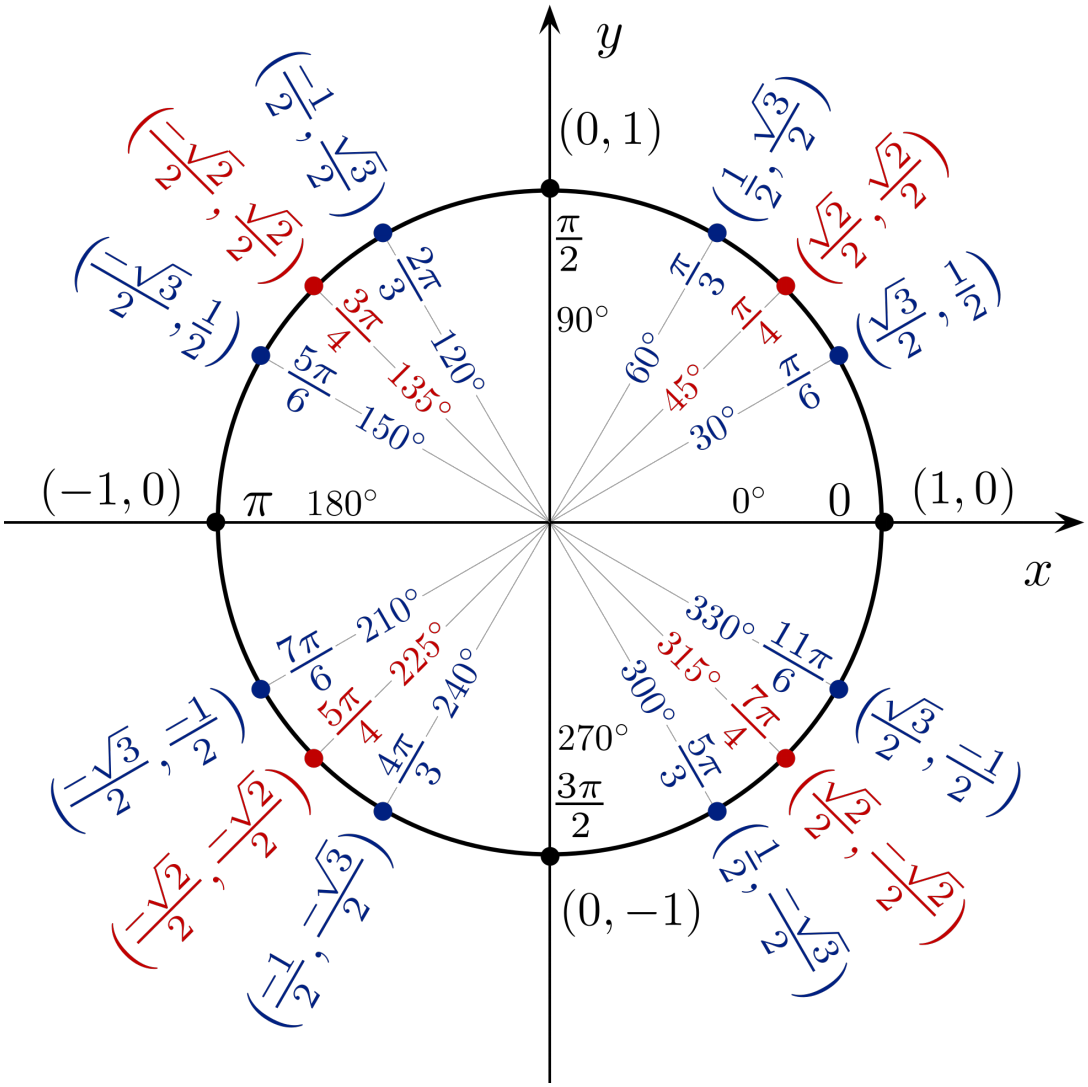
\includegraphics[scale=0.225]{sinus_cosinus}

\begin{flalign}
& \sin \Big(\frac{\pi}{2} - \alpha \Big) = \cos \alpha  & \nonumber \\
& \cos \Big( \frac{\pi}{2} + \alpha \Big) = \sin(\alpha) & \nonumber \\
& \tan \Big( \frac{\pi}{2} - \alpha \Big) = \frac{1}{\tan \alpha }& \nonumber \\
& \sin( - \alpha) = - \sin \alpha & \nonumber  \\
& \cos( - \alpha) = \cos \alpha & \nonumber  \\
& \tan(- \alpha) = - \tan \alpha & \nonumber \\
& \sin ( \alpha \pm \beta ) = \sin \alpha \cos \beta \pm \cos \alpha \sin \beta & \nonumber \\ 
& \cos( \alpha \pm \beta ) = \cos \alpha \cos \beta \mp \sin \alpha \sin \beta & \nonumber \\
& \tan( \alpha \pm \beta) = \frac{\tan \alpha \pm \tan \beta}{1 \mp \tan \alpha \tan \beta} & \nonumber \\
& \sin ( 2 \alpha) = 2 \sin \cos \alpha & \nonumber \\
& \cos( 2 \alpha) = \cos^2 \alpha - \sin^2 \alpha = 2 \cos^2 \alpha - 1 & \nonumber \\
& \tan( 2 \alpha) = \frac{2 \tan \alpha}{4 - \tan^2 \alpha} & \nonumber \\
& \sin( 3 \alpha) = 3 \sin \alpha - 4 \sin^3 \alpha & \nonumber \\
& \cos(3 \alpha) = 4 \cos^3 \alpha - \cos \alpha & \nonumber \\
& \tan(3 \alpha) = \frac{3 \tan \alpha - \tan^3 \alpha}{1 - 3 \tan^2 \alpha} & \nonumber \\
& \sin^2 \Big(\frac{\alpha}{2} \Big) = \frac{1 - \cos \alpha}{2} & \nonumber \\
& \cos^2 \Big(\frac{\alpha}{2} \Big) = \frac{1 + \cos \alpha}{2} & \nonumber  \\
& \tan^2 \Big(\frac{\alpha}{2} \Big) = \frac{1 - \cos \alpha}{1 + \cos \alpha} & \nonumber \\
& \tan \Big(\frac{\alpha}{2} \Big) = \frac{1 - \cos \alpha}{\sin \alpha} = \frac{\sin \alpha}{1 + \cos \alpha} & \nonumber \\
& \sin \alpha + \sin \beta = 2 \sin \frac{\alpha + \beta}{2} \cos \frac{\alpha - \beta}{2} & \nonumber \\
& \sin \alpha - \sin \beta = 2 \cos \frac{\alpha + \beta}{2} \sin \frac{\alpha - \beta}{2} & \nonumber \\
& \cos \alpha + \cos \beta = 2 \cos \frac{\alpha + \beta}{2} \cos \frac{\alpha - \beta}{2} & \nonumber \\
& \cos \alpha - \cos \beta = - 2 \sin \frac{\alpha + \beta}{2} \sin \frac{\alpha - \beta}{2} & \nonumber \\
& \sin \alpha \sin \beta = \frac{1}{2} [ \cos ( \alpha - \beta) - \cos (\alpha + \beta)] & \nonumber \\
& \cos \alpha \cos \beta = \frac{1}{2} [ \cos ( \alpha - \beta) + \cos( \alpha + \beta)] & \nonumber \\
& \sin \alpha \cos \beta = \frac{1}{2} [ \sin( \alpha - \beta) + \sin( \alpha + \beta) ] & \nonumber \\
& \sin( \arccos(x)) = \sqrt{1 - x^2}  & \nonumber \\
& \cos( \arcsin(x)) = \sqrt{1 - x ^2} & \nonumber
\end{flalign}

\section{Quadratic Formula}
\[ x = \frac{-b + \pm \sqrt{b^2 - 4 a c} }{2 a} \]

\section{Weitere McLaurin Reihen}
\begin{align*}
\sin(x)     &= \sum_{n=0}^{\infty} \frac{(-1)^{n}}{(2 n+1) !} x^{2 n+1} \\
            &= x-\frac{x^{3}}{6}+\frac{x^{5}}{120} - O(x^7) \\
\cos(x)     &= \sum_{n=0}^{\infty} \frac{(-1)^{n}}{(2 n) !} x^{2 n} \\
            &= 1-\frac{x^{2}}{2}+\frac{x^{4}}{24} - O(x^6) \\
\log(1+x)   &= \sum_{n=1}^{\infty}(-1)^{n+1} \frac{x^{n}}{n} \forall |x|<1 \\
            &= x-\frac{x^{2}}{2}+\frac{x^{3}}{3} - O(x^4) \\
\arcsin     &= \sum_{n=0}^{\infty} \frac{(2 n) !}{4^{n}(n !)^{2}(2 n+1)} x^{2 n+1} \\
            &= x-\frac{x^{3}}{6}+\frac{3 x^{5}}{40} + O(x^7) \\
\arccos(x)  &= \pi/2-\arcsin(x) \\
\arctan(x)  &= \sum_{n=0}^{\infty} \frac{(-1)^{n}}{(2 n+1)} x^{2 n+1} \\
            &= x-\frac{x^{3}}{3}+\frac{x^{5}}{5} - O(x^7) \\
\sinh(x)    &= \sum_{n=0}^{\infty} \frac{x^{2 n+1}}{(2 n+1) !} \\
            &= x+\frac{x^{3}}{6}+\frac{x^{5}}{120} + O(x^7) \\
\cosh(x)    &= \sum_{n=0}^{\infty} \frac{x^{2 n}}{(2 n) !} \\
            &= 1+\frac{x^{2}}{2}+\frac{x^{4}}{24} + O(x^6) \\
\arctanh(x) &= \sum_{n=0}^{\infty} \frac{x^{2 n+1}}{2 n+1} 
\end{align*}


\section{Proofs}
\Beweis[$\sin(x) < x$] Case distinction $\rightarrow$ Mean-Value-Theorem \\
$\forall x \in (0,1) \exists \xi \in (0,1)$ with
\begin{align*}
\sin^{\prime}(\xi) &= \frac{\sin(x)-\sin(0)}{x-0} \\
\cos(\xi)		&= \frac{\sin(x)}{x}
\end{align*}
Note that $\cos$ is bounded. \\

\Beweis[Fixpunkt 6.4a] Define $g(x):=f(x)-x \rightarrow$ Zwischenwertsatz \\

\Beweis[Sandwich]
\begin{enumerate}
\item $\lim\limits_{n \rightarrow \infty} a_{n} = \lim\limits_{n \rightarrow \infty} b_{n} = \alpha$ 
\item $a_{n} \leq c_{n} \leq b_{n} \ \forall n \geq K$
\end{enumerate}

\(
\text{Es gilt } \abs{a_n - \alpha} < \epsilon \implies - \epsilon < a_n - \alpha \\
\text{Es gilt } \abs{b_n - \alpha} < \epsilon \implies + \epsilon > b_n - \alpha \\
\implies - \epsilon < a_n - \alpha \leq c_n - \alpha \leq b_n - \alpha < \epsilon \\
\implies \abs{c_n - \alpha} < \epsilon \implies \lim\limits_{n \rightarrow \infty} c_{n} = \alpha
\) 

\Beweis[Hôpital]
\begin{align*}
\lim _{x \rightarrow a} \frac{f(x)}{g(x)} &=\lim _{x \rightarrow a} \frac{f(x)-f(a)}{g(x)-g(a)} \\
&=\lim _{x \rightarrow a} \frac{[f(x)-f(a)] /(x-a)}{[g(x)-g(a)] /(x-a)} \\
&=\frac{\lim _{x \rightarrow a}([f(x)-f(a)] /(x-a))}{\lim _{x \rightarrow a}([g(x)-g(a)] /(x-a))} \\
&=\frac{f^{\prime}(a)}{g^{\prime}(a)}
\end{align*}

\Beweis[Monotone Konvergenz]
\begin{enumerate}
\item Supremum exists
\item $\forall \varepsilon>0,$ there exists $N$ such that $a_{N}>c-\varepsilon$
\item \dots
\end{enumerate}

\section{Tricks}
\Trick
\begin{align*}
a^n-b^n =& (a-b)(a^{n-1} + a^{n-2} b +\dots+b^{n-1}) \\
		=& (a-b)\sum_{i=0}^{n-1} b^{i}a^{n-1-i} 
\end{align*}

\section{Rezepte}
\subsection*{Konvergenz von Reihen}
\begin{enumerate}
\item Weierstrass (monoton + beschränkt)
\item Vergleichssatz
\item Geometrische Folge
\item Alternierende Reihe
\item Riemann Zeta
\item Teleskopieren
\item $\lim \limits_{n \rightarrow \infty} a_n = 0$ ?
\item konvergiert das Integral?
\end{enumerate}

\section{Am Schluss}
\begin{itemize}
	\item 'c' nirgends vergessen?
\end{itemize}

\end{multicols*}
\end{document}
